\begin{frame}{MC efficiency (1)}
\setlength{\unitlength}{1mm}
\begin{center}
MC true events $\chi_b(3P) \to \Y1S \gamma$ (other decays have the same shape)
\begin{picture}(70,50)
      %
    \put(0,0){
      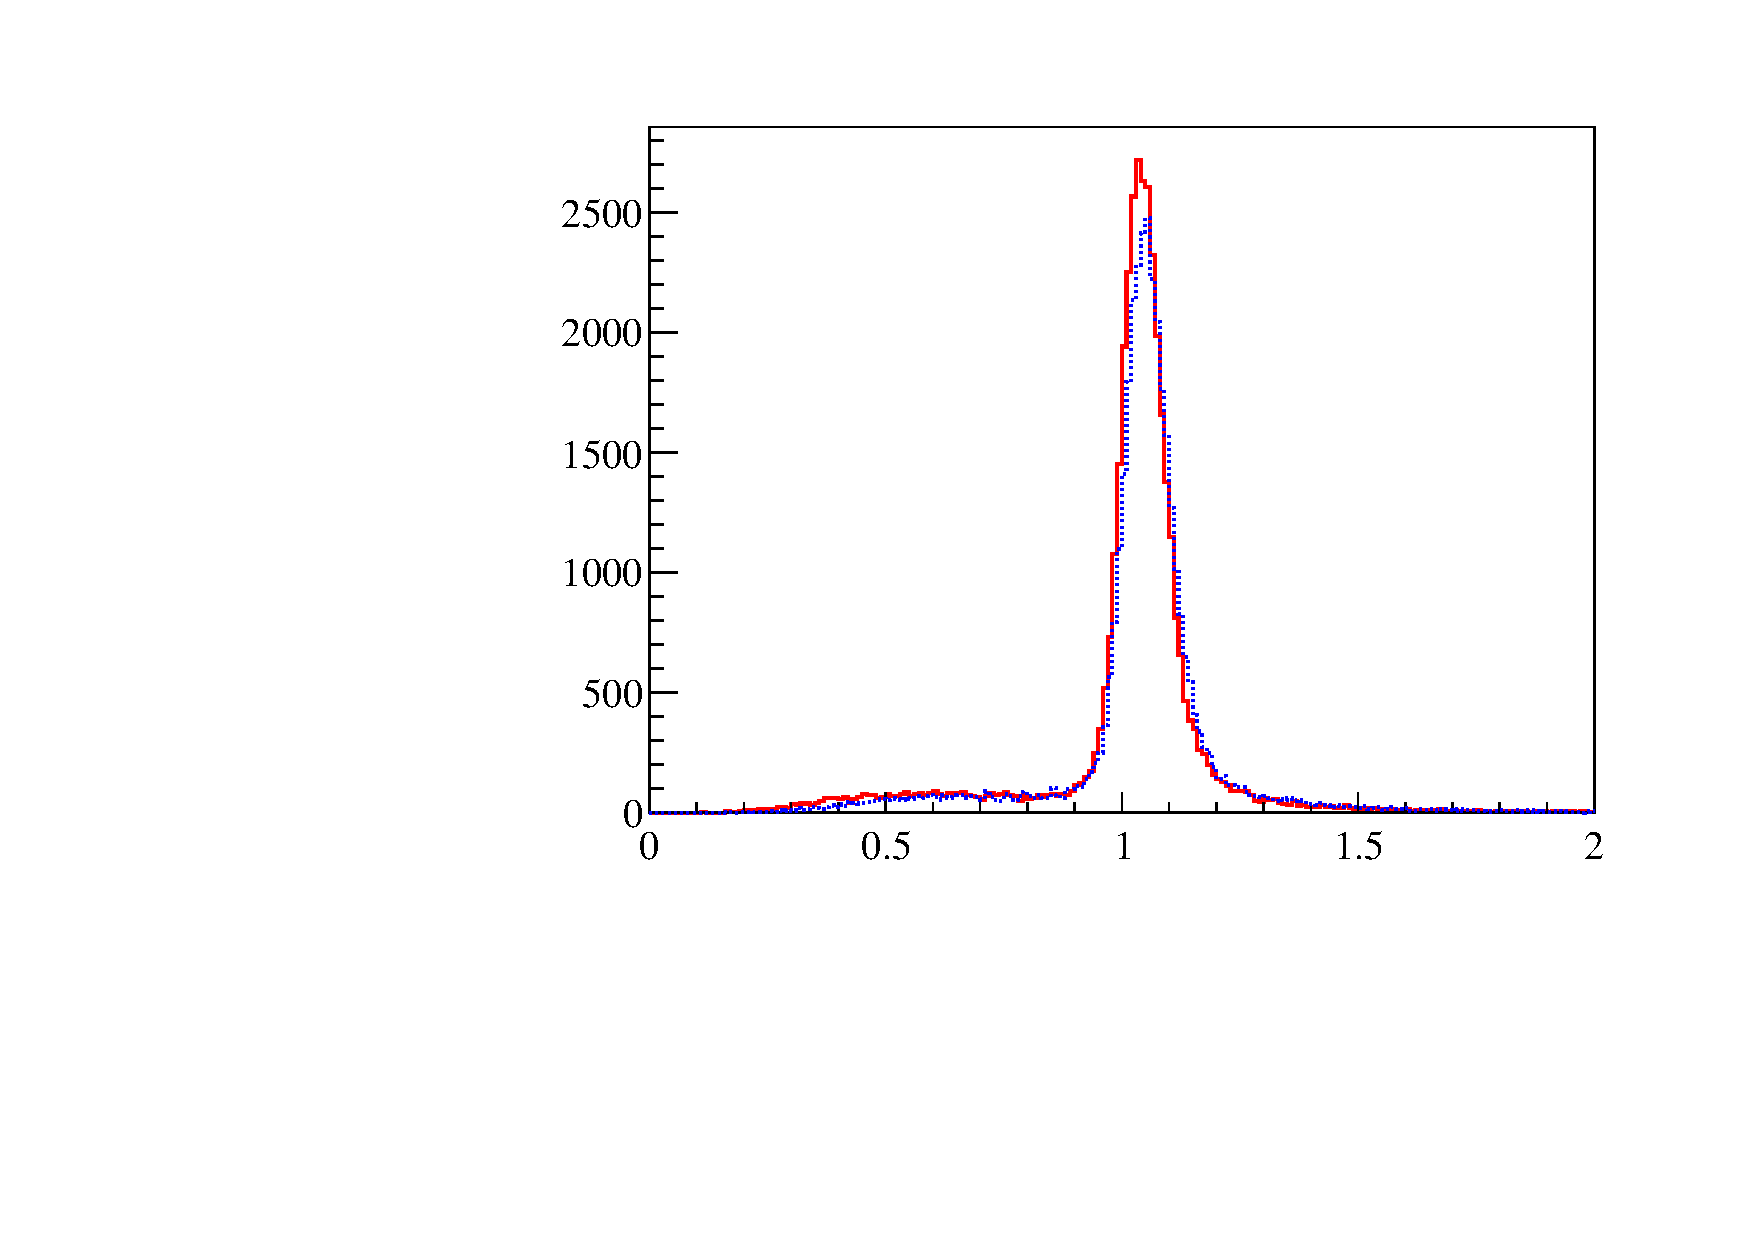
\includegraphics[width=70mm, height=50mm]{mc-fits/cb3_h}
    }
    
%    \put(0,40){
%      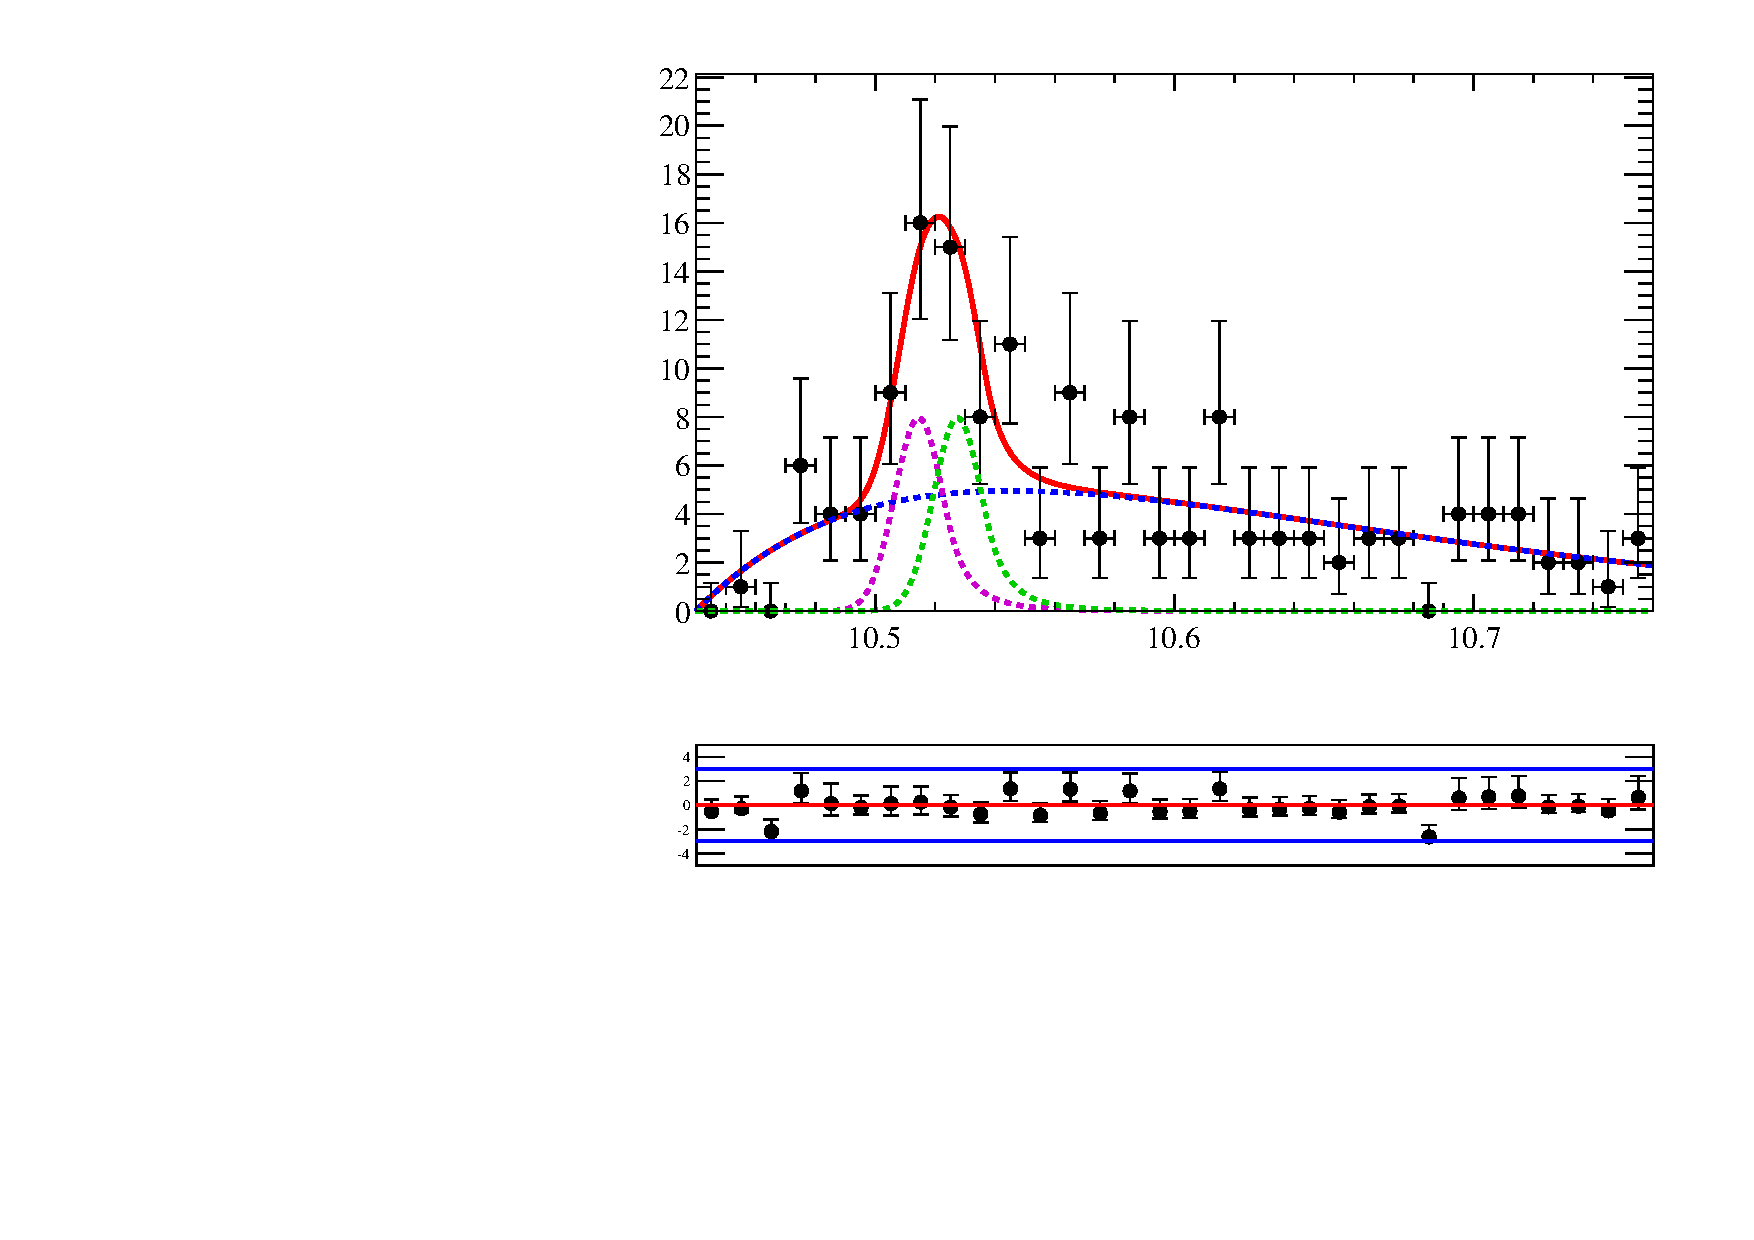
\includegraphics[width=50mm, height=40mm]{7.1-chib3s-fit/f2011_fix_27_None}
%    }

    \put(0,12){\begin{sideways}Candidates\end{sideways}}
    \put(20,0){$m_{\mumu \gamma} - m_{\mumu} \left[\gevcc\right]$}

%    
%    \put(0,55){\tiny \begin{sideways}Candidates/(20\mevcc)\end{sideways}}
%    \put(2, 49.5){\tiny $m_{\mumu \gamma} - m_{\mumu} + 10.3552 \left[\gevcc\right]$}
%    \put(25,70){$\sqrt{s} = 7 \gev$}     
%    \graphpaper[2](0,0)(70, 50)        
  \end{picture}
 \end{center}
 
\begin{alertblock}{}
\footnotesize
The flat left tails are due to photons which, although being correctly
associated to the \chib decay, are poorly reconstructed in the calorimeter. In
principle, these tails could be modeled in our fit to signal, but in practice
they will not be distinguishable from background. Therefore, the number of
\chib events for efficiency calculations \textbf{is not determined by simple event
counting but from a fit} where the tails are considered as background. $\Upsilon$
events are obtained by counting mc-true events.
\end{alertblock}

\end{frame}